\documentclass{beamer}
\usepackage[utf8]{inputenc}
\usepackage[T1]{fontenc}
\usepackage{circuitikz}

\usepackage{multirow}

\title{CS241: Hardware Design}
\date{\today}
\author[Fyfe]{Professor Charles Fyfe}
\institute{St Olaf College}

\usetheme{grape}

\usepackage{parskip}
\usepackage{multicol}
\usepackage{graphicx}

\begin{document}


\titlepage

% just sections up top
\setcounter{tocdepth}{1}

\begin{frame}{Outline}
%	\begin{multicols}{2}
		\tableofcontents
%	\end{multicols}
\end{frame}

% show subsections later
\setcounter{tocdepth}{2}


\Section{Introduction}

\begin{frame}{Course Overview}

	\includegraphics[width=\columnwidth]{images/dune-robot-hbo}

	{\center
		Thou shalt not make a machine in the likeness of a human mind
	}

	{\small \hfill
		Dune, Frank Herbert
	}
\end{frame}


\begin{frame}{Course Overview}

	Computers feel like magic. You type words. The machine does complex things. Especially in the era of large language models

	But it's not magic. Computers are made of semiconductors, metal, and magnets. Three different kinds of rocks

	This course is about demystifying the machine and exploring how, fundamentally, computers do what they do. Specifically, we'll be looking at:
	\begin{itemize}
		\item The fundamental components of a computer
		\item How data is stored on a computer
		\item Building electrical circuits to perform logic
		\item Programming in Assembly (a very low-level language)
	\end{itemize}
\end{frame}

\Subsection{Grading}

\begin{frame}{Course Grade Breakdown}
	\begin{itemize}
		\item Tests: 45\%
		\item Assignments: 45\%
		\item Participation: 10\%
	\end{itemize}
\end{frame}

\begin{frame}{Tests}
	\begin{itemize}
		\item There are eight standards in the class. Each is weighted equally
		\item There are four quizzes. Each quiz covers two standards
		\item The final covers all eight standards
		\item You only have to demonstrate proficiency once
		\item If you demonstrate proficiency on the quiz, you're good. Full credit. You can skip that part of the final
		\item If you demonstrate profociency on the final, full credit, regardless of your grade on the quiz
	\end{itemize}
\end{frame}


\begin{frame}{Assignments}
	\begin{itemize}
		\item One assignment per standard. Each weighted equally
		\item Assignment prompts are on Doenet
		\item Some work will be graded automatically by Doenet
		\item Some work you will submit as a PDF on Moodle
		\item Coding assignments will be submitted via csgit
		\item Please work together in small groups
		\item Please ensure that the work you turn in reflects your own understanding
	\end{itemize}
\end{frame}

\begin{frame}{Peer Reviews}
	\begin{itemize}
		\item Participation score (10\% of your total grade) is mostly based on peer reviews
		\item Reviews will be short. Less than one page. They should include \emph{specific examples} of ways your peers helped you succeed
		\item You can get full credit here without too much trouble. Show up. Work together. Make it easy for your peers to write nice things about you
		\item I recommend keeping notes over the course of the semester when someone is particularly helpful, insightful, etc
	\end{itemize}
\end{frame}

\Subsection{Important Links}

\begin{frame}{Important Links}
	\begin{itemize}
		\item Dive Into Systems: \url{https://diveintosystems.org/book/index.html}
		\item Doenet: \url{https://www.doenet.org/course?tool=dashboard&courseId=_GnqAk2zB64CHKPeZY9Ren}
		\item ARM Tutorial: \url{https://diveintosystems.org/book/C9-ARM64/index.html}
		\item ARM Simulator: \url{http://163.238.35.161/~zhangs/arm64simulator/}
		\item Circuitverse: \url{https://circuitverse.org/simulator}
	\end{itemize}
\end{frame}

\Subsection{Everything Else}

\begin{frame}{Everything else}
	\begin{itemize}
		\item Late work policy, AI use policy, disability accommodations, etc
		\item Please look at the syllabus
		\item I even put a table of contents in it, with links
		\item It will take you 30 seconds
	\end{itemize}
\end{frame}



\Section{Data Representation}

\begin{frame}{How do computers store information?}
	Computers work using electrical signals which can be on or off. If we let:
	\begin{itemize}
		\item On means 1
		\item Off means 0
	\end{itemize}
	We can use sequences of 0s and 1s to represent information
\end{frame}

\Subsection{Positive Integers in Binary}

\begin{frame}{Numbers in Base Ten (aka Decimal)}
	Let's start by talking about how we write numbers normally.

	For example, let's look at the number 109:
	\begin{align*}
		109 & = 100 \;+\; 0 \;+\; 9                                   \\
		    & = 1 \Times 10^2 \;+\; 0 \Times 10^1 \;+\; 9 \Times 10^0
	\end{align*}
	This way of writing numbers is called base ten.
	We use ten digits (0 to 9 inclusive) and each position in the number is scaled by a power of ten.

	In terms of math, there is nothing special about base ten. We probably use it
	because we have ten fingers. Some ancient civilizations used sompletely
	different systems for counting!
\end{frame}

\begin{frame}{Numbers in Base Two (aka Binary)}
	Computers don't have fingers. They express everything as sequences of 1s and 0s. This format is called binary:

	\begin{align*}
		0b1101101 & =
		1 \Times 2^6 +
		1 \Times 2^5 +
		0 \Times 2^4 +
		1 \Times 2^3 +
		1 \Times 2^2 +
		0 \Times 2^1 +
		1 \Times 2^0                              \\
		          & = 64 + 32 + 0 + 8 + 4 + 0 + 1 \\
		          & = 109                         \\
	\end{align*}
	Importantly: we always use the prefix ``0b'' to avoid confusion when writing numbers in binary.

	1101 is one thousand one hundred and one

	0b1101 is thirteen
\end{frame}

\begin{frame}{Converting from Decimal to Binary}

	If the number is odd, append a 1 on the left. Otherwise, append a 0. Then
	divide your decimal number by two and ignore any remainder. Repeat until your
	decimal number is zero. \\

	For example, starting with 58:

	\begin{itemize}
		\item 58 is even, so append \Highlight{0}. Divide by two, leaving 29.
		\item 29 is odd, so append \Highlight{1}0. Divide by two, leaving 14.
		\item 14 is even, so append \Highlight{0}10. Divide by two, leaving 7.
		\item 7 is odd, so append \Highlight{1}010. Divide by two, leaving 3.
		\item 3 is odd, so append \Highlight{1}1010. Divide by two, leaving 1.
		\item 1 is odd, so append \Highlight{1}11010. Divide by two, leaving 0.
	\end{itemize}

	So 58 in binary is 0b111010.

\end{frame}

\begin{frame}{Converting from Binary to Decimal}

	We can confirm by converting back. The rightmost bit is worth 1, then 2, then
	4, and so on:

	\begin{align*}
		0b111010 & =
		1 \Times 2^5 +
		1 \Times 2^4 +
		1 \Times 2^3 +
		0 \Times 2^2 +
		1 \Times 2^1 +
		0 \Times 2^0                          \\
		         & = 32 + 16  + 8 + 0 + 2 + 0 \\
		         & = 58
	\end{align*}

\end{frame}

\begin{frame}{Addition in Binary}
	Binary addition works just like decimal addition.
	Start from the right, add straight down, and carry when you run out of digits.

	For example:
	\[
		\begin{array}{ccccccccc}
			1 & 1 & 1 & 1 & 1 &   &   &   &   \\
			  & 0 & 0 & 1 & 1 & 1 & 0 & 0 & 0 \\
			+ & 1 & 1 & 1 & 0 & 1 & 0 & 0 & 1 \\
			\hline
			1 & 0 & 0 & 1 & 0 & 0 & 0 & 0 & 1 \\
		\end{array}
	\]

	What happens if we try to perform this operation but we only have 8 bits to
	store the answer?
\end{frame}

\begin{frame}{Multiplication in Binary}
	Binary multiplication works just like decimal multiplication.
	Multiply the top number by the rightmost digit of the bottom number.
	Then move to the next line, add a zero, and repeat for the next digit.
	Finally, add up the lines. For example:
	\[
		\begin{array}{cccccc}
			  &   &        & 1 & 1 & 0 \\
			  &   & \times & 1 & 0 & 1 \\
			\hline
			  &   &        & 1 & 1 & 0 \\
			  &   & 0      & 0 & 0 & 0 \\
			+ & 1 & 1      & 0 & 0 & 0 \\
			\hline
			  & 1 & 1      & 1 & 1 & 0 \\
		\end{array}
	\]
\end{frame}

\begin{frame}{Division in Binary}
	To divide by 2, shift the bits one place to the right. \\

	To divide by 4, shift the bits two places to the right. \\

	That's about as deep as we go in this class. If you're curious to learn more,
	see the textbook.

\end{frame}



\Subsection{Hexadecimal}

\begin{frame}{What? Why?}

	Binary is how machines store data. But writing out binary by hand is a chore.
	In practice, it's often convenient to use hexadecimal (base 16) instead.

	\begin{itemize}
		\item Decimal uses ten digits, 0-9
		\item Binary uses two digits, 0 and 1
		\item Hexadecimal uses sixteen digits: 0-9 along with A-F
	\end{itemize}
	Hexadecimal values are always prefixed with ``0x'' to avoid ambiguity.
\end{frame}

\begin{frame}{Converting Between Binary and Hexadecimal}

	Converting back and forth between binary and hexadecimal does not require any
	math! Every four bits become one hex digit.
	\begin{align*}
		0b0000 & = 0x0 = 0 & 0b1000 & = 0x8 = 8  \\
		0b0001 & = 0x1 = 1 & 0b1001 & = 0x9 = 9  \\
		0b0010 & = 0x2 = 2 & 0b1010 & = 0xA = 10 \\
		0b0011 & = 0x3 = 3 & 0b1011 & = 0xB = 11 \\
		0b0100 & = 0x4 = 4 & 0b1100 & = 0xC = 12 \\
		0b0101 & = 0x5 = 5 & 0b1101 & = 0xD = 13 \\
		0b0110 & = 0x6 = 6 & 0b1110 & = 0xE = 14 \\
		0b0111 & = 0x7 = 7 & 0b1111 & = 0xF = 15 \\
	\end{align*}
\end{frame}

\begin{frame}{Converting Hexadecimal to Decimal}

	Hexadecimal is base 16. So each place corresponds to a power of 16.

	\begin{align*}
		0x3AB & = 3 \times 16^2 + 10 \times 16^1 + 11 \times 16^0 \\
		      & = 3 \times 256 + 10 \times 16 + 11 \times 1       \\
		      & = 768 + 160 + 11                                  \\
		      & = 954                                             \\
	\end{align*}

	Hexadecimal is very compact! These numbers get big fast

\end{frame}

\begin{frame}{Arithmetic in Hexadecimal}

	Addition and multiplication work in hexadecimal just like they do in binary and
	decimal. Just be careful about carrying.

	\[
		\begin{array}{ccccc}
			1 &   &   & 1 &   \\
			  & 4 & 1 & 7 & B \\
			+ & C & 2 & 0 & F \\
			\hline
			1 & 0 & 3 & 8 & A \\
		\end{array}
	\]

\end{frame}






\Subsection{Negatives in Binary}

\begin{frame}{First Attempt: Signed Magnitude}

	We can use the first digit to hold the sign, then the rest of the digits to
	hold magnitue:

	\begin{itemize}
		\item 0b\Highlight{0}1011001 is positive 10110001, so 89
		\item 0b\Highlight{1}1011001 is negative 1011001, so -89
	\end{itemize}

	This is nice and straightforward!

\end{frame}

\begin{frame}{Addition and Subtraction with Signed Magnitude}
	Adding positive numbers works just the same. But what happens if we throw a minus sign in there?

	For example, let's look at 12 - 5. First, rewrite it as 12 + (-5). Then:

	\[
		\begin{array}{ccccccccc}
			  & 0 & 0 & 0 & 0 & 1 & 1 & 0 & 0 \\
			+ & 1 & 0 & 0 & 0 & 0 & 1 & 0 & 1 \\
			\hline
			  & ? & ? & ? & ? & ? & ? & ? & ? \\
		\end{array}
	\]

	We know the result should be 7 (0b00000111). But our regular rules for addition
	do not get us there.
\end{frame}

\begin{frame}{Zero with Signed Magnitude}

	Using signed magnitude, 0b00000000 is zero.

	And 0b10000000 is negative zero (which is also zero).

	Using this convention, we have to worry about the difference between numerical
	equality and bitwise equality. That seems pretty messy.
\end{frame}

\begin{frame}{Can We Do Better?}
	Signed magnitude was a swing and a miss. What do we want when we talk about negative numbers?
	\begin{itemize}
		\item We want positive numbers to work like we expect
		\item We want 0b00000000 to be zero, with no ambiguity
		\item We want addition and subtraction to work the same for positive and negative
	\end{itemize}
\end{frame}

\begin{frame}{Another Idea: Two's Complement}
	We know 1 - 1 = 0. Put another way, 1 + (-1) = 0. Can we work backwards from there to figure out how to write -1?
	\[
		\begin{array}{ccccccccc}
			  & 0 & 0 & 0 & 0 & 0 & 0 & 0 & 1 \\
			+ & 1 & 1 & 1 & 1 & 1 & 1 & 1 & 1 \\
			\hline
			  & 0 & 0 & 0 & 0 & 0 & 0 & 0 & 0 \\
		\end{array}
	\]

	Remember: on a computer, our numbers have to fit in a set number of bits.
	Anything past that gets thrown away. This is called overflow. In this case,
	overflow works in our favor!
\end{frame}

\begin{frame}{Working Backwards from Zero}
	We can use the same trick to identify the rest of the negative numbers:
	\begin{itemize}
		\item 0b00000000 is 0
		\item 0b11111111 is -1
		\item 0b11111110 is -2
		\item 0b11111101 is -3
		\item 0b11111100 is -4
		\item etc
	\end{itemize}

\end{frame}

\begin{frame}{The Sign Bit (Again)}
	We only have 256 possible integers. How do we decide where the positives end and the negatives begin?

	Unsigned int: bits are worth 1, 2, 4, 8, 16, 32, 64, 128

	Signed magnitude: bits are worth $\pm1, \pm2, \pm4, \pm8, \pm16, \pm32, \pm64$,
	and the last bit tells us whether to use positive or negative (yikes)

	Two's complement: bits are worth 1, 2, 4, 8, 16, 32, 64, \Highlight{-128}

	Range of possible values is -128 to 127.
\end{frame}

\begin{frame}{Flipping Signs in Two's Complement}
	To flip the sign of a two's complement integer, flip all the bits then add 1. Ignore the overflow (if any). This works for both positive and negative numbers.

	For example:
	\begin{itemize}
		\item 55 is 0b01010111
		\item Flip the bits: 0b10101000, then add 1: 0b10101001
		\item So -55 is 0b10101001
		\item Flip the bits again: 0b01010110, add 1: 0b01010111
		\item So -(-55) = 55 = 0b01010111
	\end{itemize}

	What happens if we negate zero?
\end{frame}

\begin{frame}{Overflow}
	Overflow is important for two's complement. It ensures that positive zero and negative zero are the same. But it is also a constraint!

	Try adding 0b01101001 + 0b01011010:
	\[
		\begin{array}{ccccccccc}
			  &   & 1 & 1 & 1 &   &   &   &   \\
			  & 0 & 1 & 1 & 0 & 1 & 0 & 0 & 1 \\
			+ & 0 & 1 & 0 & 1 & 1 & 0 & 1 & 0 \\
			\hline
			  & 1 & 1 & 0 & 0 & 0 & 0 & 1 & 1 \\
		\end{array}
	\]

	These are two's complement numbers. Convert them to decimal. What just
	happened?

\end{frame}


\Subsection{Fractions and Decimals}

\begin{frame}{The Decimal Point}

	Sometimes we need to store numbers that aren't integers. \\

	Before we worry about binary, what does 21.867 mean? \\

	\begin{align*}
		21.867 & = 2 \Times 10^1 + 1 \Times 10^0 + 8 \Times ?? + 6 \Times ?? + 7 \Times ??
	\end{align*}

\end{frame}

\begin{frame}{The Decimal Point}

	In decimal:
	\begin{align*}
		21.867 & = 2 \Times 10^1 + 1 \Times 10^0 + 8 \Times 10^{-1} + 6 \Times 10^{-2} + 7 \Times 10^{-3}             \\
		       & =2 \Times 10 + 1 \Times 1 + 8 \Times \frac{1}{10} + 6 \Times \frac{1}{100} + 7 \Times \frac{1}{1000} \\
	\end{align*}

	In binary, we can use the same idea:
	\begin{align*}
		0b101.010 & = 1 \Times 2^2 + 0 \Times 2^1 + 1 \Times 2^0 + 0 \Times 2^{-1} + 1 \Times 2^{-2} + 0 \Times 2^{-3} \\
		          & = 1 \Times 4 + 0 + 1 \Times 1 + 0 + 1 \Times \frac{1}{4} + 0                                       \\
		          & = 5.25                                                                                             \\
	\end{align*}

\end{frame}

\begin{frame}{Fixed Point Representation}

	The computer just stores 1s and 0s, not decimal points. How do we distinguish
	these values?
	\begin{itemize}
		\item 0b0101110.1 = 46.5
		\item 0b010111.01 = 23.25
		\item 0b01011.101 = 11.625
	\end{itemize}

	One option is to specify the location of the decimal point ahead of time. For
	example, we could say that our eight-bit binary decimal always has two decimal
	bits. \\

	What is an upside of this approach? What is a downside?

\end{frame}

\begin{frame}{Floating Point Representation}

	Floating point numbers are a bit more complicated, but much more flexible. For
	a 16-bit floating point number we get:

	\begin{itemize}
		\item 1 bit for the sign
		\item 5 bits for the exponent (value -14 to 15)
		\item 10 bits for the significand (value 0 to 1023)
	\end{itemize}

	To turn those components into a value we use:
	\begin{align*}
		\text{value} & = (-1)^{\text{sign}} \times 2^{\text{exponent} - 15} \times \left(1 + \frac{\text{significand}}{1024} \right)
	\end{align*}

	Why offset the exponent?

	Why add 1 to the significand fraction?

\end{frame}

% Explanation here for the 127 offset: https://www.quora.com/Why-do-we-add-127-to-the-exponent-in-IEEE-754-floating-number-format-to-get-the-actual-exponent-value

\begin{frame}{Floating Point Examples}

	\begin{align*}
		\underbrace{0}_\text{sign} \; \underbrace{01111}_\text{exponent} \; \underbrace{0000000000}_\text{significand} & = (-1)^0 \times 2^{15 - 15} \times \left( 1 + \frac{0}{1024} \right) \\
		                                                                                                               & = 1 \times 2^0   \times \left( 1 + 0 \right)                         \\
		                                                                                                               & = 1                                                                  \\
	\end{align*}
	\begin{align*}
		0 \; 01101 \; 0101010101 & = (-1)^0 \times 2^{13 - 15} \times \left( 1 + \frac{341}{1024} \right) \\
		                         & \approx 0.33325195                                                     \\
	\end{align*}
	\begin{align*}
		1 \; 11110 \; 1111111111 & = (-1)^1 \times 2^{30 - 15} \times \left( 1 + \frac{1023}{1024} \right) \\
		                         & = -65504                                                                \\
	\end{align*}

	Why
\end{frame}

\begin{frame}{Floating Point Special Cases}

	\[
		\begin{array}{ccccr}
			0 & 00000 & 0000000000     & = 0          \\
			1 & 00000 & 0000000000     & = -0         \\
			0 & 11111 & 0000000000     & = \infty     \\
			1 & 11111 & 0000000000     & = -\infty    \\
			0 & 11111 & \text{nonzero} & = \text{NaN} \\
		\end{array}
	\]

	There's more to it than this. If you're curious, read up on subnormal numbers
	\href{https://en.wikipedia.org/wiki/Half-precision_floating-point_format}{here}

\end{frame}

\begin{frame}{Floating Point for Big Integers}

	If we're dealing with big numbers, floating point often works better than fixed
	point. This is true even if both formats use the same number of bits.

	\begin{itemize}
		\item 8-bit unsigned integer: max value 255
		\item 16-bit unsigned integer: max value 65,535
		\item 32-bit unsigned integer: max value 4.2 billion % 4,294,967,295
		\item 16-bit floating point: max value 65,504 (also handles negatives, fractions)
		\item 32-bit floating point: max value 340 billion billion billion billion (also handles negatives, fractions)
		      % 340,282,346,638,528,859,811,704,183,484,516,925,440 
	\end{itemize}

\end{frame}

\begin{frame}{Floating Point Limitations}

	So what's the catch?

\end{frame}

%        \item Convert 0b100110.10 from fixed-point binary to decimal.
%        \item Convert 23.75 from decimal to fixed-point binary.
%        \item Add fixed-point binary numbers 0b101101.01 + 0b010011.11. Convert to decimal to confirm your result.
%        \item Show that the 16-bit floating point expression ${1 \; 01000 \; 1100000000}$ is equal to -3.5 in decimal.

\Subsection{Beyond Numbers}

\begin{frame}{What else do computers store?}
	There are many cases where we want a computer to store non-numerical data:
	\begin{itemize}
		\item Text
		\item Colors
		\item Sounds
		\item Images
		\item Videos
		\item Websites
		\item Multiple things at once
	\end{itemize}
\end{frame}

\begin{frame}{Characters and Strings}
	\begin{itemize}
		\item Each character is represented by a number
		\item The most straightforward encoding is ASCII
		\item Modern use cases typically use Unicode (much bigger)
		\item To make a string, put a bunch of characters in a row
		\item Question: how do we identify the end of a string?
	\end{itemize}
\end{frame}

\begin{frame}{ASCII Table}
	\includegraphics[width=\columnwidth]{images/ascii-table}
\end{frame}

\begin{frame}{Colors and Images}
	\begin{itemize}
		\item A color can be described by three numbers (R, G, B)
		\item We can represent an image as a grid of colored pixels
		\item Question: do we need a null byte at the end of a pixel/row/image? Why or why not?
	\end{itemize}
	\includegraphics[width=\columnwidth]{images/mario-pixels}
\end{frame}

\begin{frame}{Sound}
	\begin{itemize}
		\item Sound is pressure vibrations in the air
		\item We can create sound by moving a speaker cone rapidly
		\item To store sound, store the movement of the speaker cone
	\end{itemize}
	\includegraphics[width=0.5\columnwidth]{images/speakers}
\end{frame}

\begin{frame}{Structured Data}
	\begin{itemize}
		\item When you go to a website, how does your browser know what to display?
		\item When you add an item to your online cart, what data is sent?
	\end{itemize}
	\begin{columns}
		\begin{column}{0.5\textwidth}
			\includegraphics[width=\columnwidth]{images/html-example}
		\end{column}
		\begin{column}{0.5\textwidth}
			\includegraphics[width=\columnwidth]{images/json-example}
		\end{column}
	\end{columns}
\end{frame}











\Section{Logic Representation}




\Subsection{Truth Tables} % aka boolean logic

\begin{frame}{Bit Operations}
\end{frame}

\Subsection{Logic Gates}

\begin{frame}{Logic Gates: NOT}
	\begin{columns}
		\begin{column}{0.5\textwidth}
			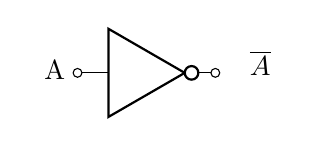
\begin{tikzpicture}
				% Paths, nodes and wires:
				\node[ieeestd not port] at (12.877, 10.375){};
				\node[ocirc] at (12, 10.375){};
				\node[ocirc] at (13.75, 10.375){};
				\node[shape=rectangle, minimum width=0.354cm, minimum height=0.59cm] at (11.555, 10.437){} node[anchor=north west, align=left, text width=-0.034cm, inner sep=6pt] at (11.36, 10.75){A};
				\node[shape=rectangle, minimum width=0.744cm, minimum height=0.59cm] at (14.36, 10.563){} node[anchor=north west, align=left, text width=0.356cm, inner sep=6pt] at (13.971, 10.875){$\overline{\text{A}}$};
			\end{tikzpicture}
		\end{column}
		\begin{column}{0.5\textwidth}
			\begin{center}
				\begin{table}[]
					\begin{tabular}{c c}
						A & $\overline{\text{A}}$ \\
						\hline
						1 & 0                     \\
						1 & 0                     \\
						0 & 1                     \\
						0 & 1
					\end{tabular}
				\end{table}
			\end{center}
		\end{column}
	\end{columns}
\end{frame}



\begin{frame}{Logic Gates: AND, NAND}
	\begin{columns}
		\begin{column}{0.5\textwidth}
			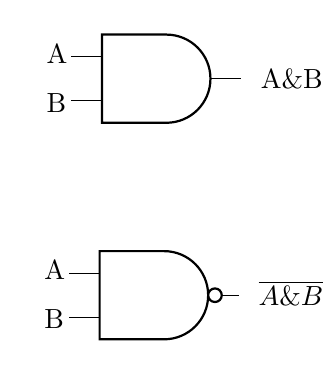
\begin{tikzpicture}
				% Paths, nodes and wires:
				\node[ieeestd and port] at (1.11, 10.22){};
				\node[ieeestd nand port] at (1.081, 7.47){};
				\node[shape=rectangle, minimum width=0.215cm, minimum height=0.59cm] at (-0.375, 10.563){} node[anchor=north west, align=left, text width=-0.173cm, inner sep=6pt] at (-0.5, 10.875){A};
				\node[shape=rectangle, minimum width=0.215cm, minimum height=0.465cm] at (-0.375, 10){} node[anchor=north west, align=left, text width=-0.173cm, inner sep=6pt] at (-0.5, 10.25){B};
				\node[shape=rectangle, minimum width=0.215cm, minimum height=0.59cm] at (-0.404, 7.813){} node[anchor=north west, align=left, text width=-0.173cm, inner sep=6pt] at (-0.529, 8.125){A};
				\node[shape=rectangle, minimum width=0.215cm, minimum height=0.465cm] at (-0.404, 7.25){} node[anchor=north west, align=left, text width=-0.173cm, inner sep=6pt] at (-0.529, 7.5){B};
				\node[shape=rectangle, minimum width=0.744cm, minimum height=0.59cm] at (2.61, 10.25){} node[anchor=north west, align=left, text width=0.356cm, inner sep=6pt] at (2.221, 10.563){A\&B};
				\node[shape=rectangle, minimum width=0.744cm, minimum height=0.59cm] at (2.581, 7.563){} node[anchor=north west, align=left, text width=0.356cm, inner sep=6pt] at (2.192, 7.875){$\overline{\text{A\&B}}$};
			\end{tikzpicture}
		\end{column}
		\begin{column}{0.5\textwidth}
			\begin{center}
				\begin{table}[]
					\begin{tabular}{c c c c}
						A & B & A\&B & $\overline{\text{A\&B}}$ \\
						\hline
						1 & 1 & 1    & 0                        \\
						1 & 0 & 0    & 1                        \\
						0 & 1 & 0    & 1                        \\
						0 & 0 & 0    & 1
					\end{tabular}
				\end{table}
			\end{center}
		\end{column}
	\end{columns}
\end{frame}




\begin{frame}{Logic Gates: OR, NOR}
	\begin{columns}
		\begin{column}{0.5\textwidth}
			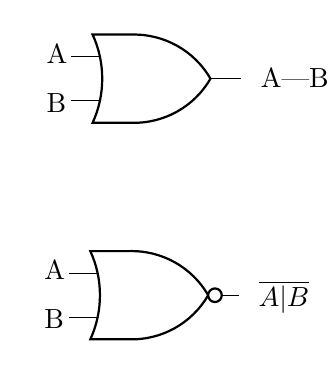
\begin{tikzpicture}
				% Paths, nodes and wires:
				\node[ieeestd or port] at (1.11, 10.22){};
				\node[ieeestd nor port] at (1.081, 7.47){};
				\node[shape=rectangle, minimum width=0.215cm, minimum height=0.59cm] at (-0.375, 10.563){} node[anchor=north west, align=left, text width=-0.173cm, inner sep=6pt] at (-0.5, 10.875){A};
				\node[shape=rectangle, minimum width=0.215cm, minimum height=0.465cm] at (-0.375, 10){} node[anchor=north west, align=left, text width=-0.173cm, inner sep=6pt] at (-0.5, 10.25){B};
				\node[shape=rectangle, minimum width=0.215cm, minimum height=0.59cm] at (-0.404, 7.813){} node[anchor=north west, align=left, text width=-0.173cm, inner sep=6pt] at (-0.529, 8.125){A};
				\node[shape=rectangle, minimum width=0.215cm, minimum height=0.465cm] at (-0.404, 7.25){} node[anchor=north west, align=left, text width=-0.173cm, inner sep=6pt] at (-0.529, 7.5){B};
				\node[shape=rectangle, minimum width=0.744cm, minimum height=0.59cm] at (2.61, 10.25){} node[anchor=north west, align=left, text width=0.356cm, inner sep=6pt] at (2.221, 10.563){A|B};
				\node[shape=rectangle, minimum width=0.744cm, minimum height=0.59cm] at (2.581, 7.563){} node[anchor=north west, align=left, text width=0.356cm, inner sep=6pt] at (2.192, 7.875){$\overline{\text{A|B}}$};
			\end{tikzpicture}
		\end{column}
		\begin{column}{0.5\textwidth}
			\begin{center}
				\begin{table}[]
					\begin{tabular}{c c c c}
						A & B & A|B & $\overline{\text{A|B}}$ \\
						\hline
						1 & 1 & 1    & 0                        \\
						1 & 0 & 1    & 0                        \\
						0 & 1 & 1    & 0                        \\
						0 & 0 & 0    & 1
					\end{tabular}
				\end{table}
			\end{center}
		\end{column}
	\end{columns}
\end{frame}


\begin{frame}{Logic Gates: XOR, XNOR}
	\begin{columns}
		\begin{column}{0.5\textwidth}
			\begin{tikzpicture}
				% Paths, nodes and wires:
				\node[ieeestd xor port] at (1.11, 10.22){};
				\node[ieeestd xnor port] at (1.081, 7.47){};
				\node[shape=rectangle, minimum width=0.215cm, minimum height=0.59cm] at (-0.375, 10.563){} node[anchor=north west, align=left, text width=-0.173cm, inner sep=6pt] at (-0.5, 10.875){A};
				\node[shape=rectangle, minimum width=0.215cm, minimum height=0.465cm] at (-0.375, 10){} node[anchor=north west, align=left, text width=-0.173cm, inner sep=6pt] at (-0.5, 10.25){B};
				\node[shape=rectangle, minimum width=0.215cm, minimum height=0.59cm] at (-0.404, 7.813){} node[anchor=north west, align=left, text width=-0.173cm, inner sep=6pt] at (-0.529, 8.125){A};
				\node[shape=rectangle, minimum width=0.215cm, minimum height=0.465cm] at (-0.404, 7.25){} node[anchor=north west, align=left, text width=-0.173cm, inner sep=6pt] at (-0.529, 7.5){B};
				\node[shape=rectangle, minimum width=0.744cm, minimum height=0.59cm] at (2.61, 10.25){} node[anchor=north west, align=left, text width=0.356cm, inner sep=6pt] at (2.221, 10.563){A{\textasciicircum}B};
				\node[shape=rectangle, minimum width=0.744cm, minimum height=0.59cm] at (2.581, 7.563){} node[anchor=north west, align=left, text width=0.356cm, inner sep=6pt] at (2.192, 7.875){$\overline{\text{A{\textasciicircum}B}}$};
			\end{tikzpicture}
		\end{column}
		\begin{column}{0.5\textwidth}
			\begin{center}
				\begin{table}[]
					\begin{tabular}{c c c c}
						A & B & A{\textasciicircum}B & $\overline{\text{A{\textasciicircum}B}}$ \\
						\hline
						1 & 1 & 0    & 1                        \\
						1 & 0 & 1    & 0                        \\
						0 & 1 & 1    & 0                        \\
						0 & 0 & 0    & 1
					\end{tabular}
				\end{table}
			\end{center}
		\end{column}
	\end{columns}
\end{frame}




\begin{frame}{Logic Circuits}

written function to a circuit diagram

\\

circuit diagram to a written function


\end{frame}




\begin{frame}{Exercises}

    \begin{enumerate}
        \item Draw a logic circuit for the boolean function 
        $f(A, B) = (A \textasciicircum B) \; | \; (A \& B)$

        \item Write out the truth table for the boolean function
        $f(A, B) = (A|B) \; \& \; (\overline{A\&B})$. Do you recognize it?
        
    \end{enumerate}
\end{frame}





\begin{frame}{Control Circuits}

	multiplexers
\end{frame}





\Section{Hardware Components}

\begin{frame}{concepts}
	\begin{itemize}
		\item Von Neumann architecture
		\item Von Neumann bottleneck
		\item clock-driven execution
	\end{itemize}
\end{frame}


\begin{frame}{image}
	\includegraphics[width=\columnwidth]{images/von-neumann-architecture.png}
\end{frame}






\Subsection{The CPU}

\Subsection{Main Memory}

\Subsection{Memory Hierarchy}



\begin{frame}{The Memory Hierarchy}
	\includegraphics[width=\columnwidth]{images/memory-hierarchy-books.png}
\end{frame}

\begin{frame}{The Memory Hierarchy}
	\includegraphics[width=\columnwidth]{images/memory-hierarchy.png}
\end{frame}



\begin{frame}{What is a cache?}

	\begin{itemize}
		\item Cache holds data that you are likely to want soon. Recent and/or adjacent.
		\item A CPU generally has a few layers of cache.
		\item Caching is also an important concept for distributed systems. Your browser caches data locally to avoid duplicate slow network requests.
	\end{itemize}

\end{frame}


\input{sections/04-assembly-fundamentals.tex}

\Section{Instruction Pipelining}

\Subsection{FDEW Cycle}

\Subsection{Pipelining}

\Subsection{Hazards}


\Section{Assembly Functions}


\begin{frame}{Push and Pop}

	When a program starts running, the OS loads the instructions into memory.

	It also allocates memory for the program to use during execution

	There is a special register called the stack pointer which provides the location of that memory

\end{frame}





\begin{frame}{Working Memory}
	\begin{columns}
		\begin{column}{0.5\textwidth}

			we do not know what piece of memory the OS will provide

			arbitrarily say it starts at 0x5000

			stack pointer points to the "bottom" of our available memory. we work our way "up" by subtracting from the stack pointer

		\end{column}
		\begin{column}{0.5\textwidth}
			\begin{alltt}
				\begin{tabular}{ r | l }
					0x4ff8 & \vdots           \\
					0x4ffc & available        \\
					0x5000 & available        \\
					0x5004 & in use by parent \\
					0x5008 & in use by parent \\
					0x500c & \vdots           \\
				\end{tabular}
			\end{alltt}
		\end{column}
	\end{columns}

\end{frame}


\begin{frame}{Branch and Link}

	New command: BL

	Branch and Link

	Branch = modify PC. Recall: PC tells us what to do next. Usually we just do the next line. In this case, we will jump to some other part of the program. This is how we call a function.

	Link = set LR to the PC of the next line. Once we're done with the function, this is how we return to the parent context.

\end{frame}


\begin{frame}{Stack Frame Walkthrough}
	\small
	\begin{columns}
		\begin{column}{0.5\textwidth}
			\begin{alltt}
				\begin{tabular}{r | l}
					       & {\quad}.section .rodata \\
					       &                         \\
					       & {\quad}.text            \\
					       & func:                   \\
					0x3fd4 & {\quad}push \{fp, lr\}  \\
					0x3fd8 & {\quad}add fp, sp, \#4  \\
					0x3fdc & {\quad}sub sp, sp, \#8  \\
					0x3fe0 & {\quad}...              \\
					0x3fe4 & {\quad}sub sp, fp, \#4  \\
					0x3fe8 & {\quad}pop \{fp, pc\}   \\
					       &                         \\
					       & {\quad}.global main     \\
					       & main:                   \\
					0x3fec & {\quad}push \{fp, lr\}  \\
					0x3ff0 & {\quad}add fp, sp, \#4  \\
					0x3ff4 & {\quad}sub sp, sp, \#12 \\
					0x3ff8 & {\quad}bl func          \\
					0x3ffc & {\quad}sub sp, fp, \#4  \\
					0x4000 & {\quad}pop \{fp, pc\}   \\
				\end{tabular}
			\end{alltt}
		\end{column}
		\begin{column}{0.5\textwidth}
			\begin{alltt}
				\begin{tabular}{ r | l}
					\vdots & \vdots    \\
					0x4ffc & available \\
					0x5000 & available \\
					0x5004 & in use    \\
					\vdots & \vdots    \\
				\end{tabular}
			\end{alltt}

			\vspace{1cm}

			\begin{alltt}
				\begin{tabular}{ r | l}
					sp & 0x5004    \\
					fp & parent fp \\
					pc & 0x3fec    \\
					lr & parent lr \\
				\end{tabular}
			\end{alltt}
		\end{column}
	\end{columns}

\end{frame}




\Section{Assembly Conditionals and Loops}



\Section{Appendix}


\Subsection{Raspberry Pi Setup}


\begin{frame}{Pi Setup: Kit Contents}
	\begin{columns}
		\begin{column}{0.5\textwidth}
			\begin{enumerate}
				\item Pi case
				\item Raspberry Pi (in box)
				\item Heat sinks
				\item Power cord
				\item Ethernet to USB adapter
				\item Ethernet cord
				\item USB 2 to USB 3 adapter
				\item SD Card
				\item Accessory case
			\end{enumerate}
		\end{column}
		\begin{column}{0.5\textwidth}
			\includegraphics[width=\columnwidth]{images/pi-kit-contents}
		\end{column}
	\end{columns}
\end{frame}


\begin{frame}{Pi Setup: Apply Heat Sinks}
	\begin{columns}
		\begin{column}{0.5\textwidth}
			\includegraphics[width=\columnwidth]{images/pi-heat-sinks-1}
		\end{column}
		\begin{column}{0.5\textwidth}
			\includegraphics[width=\columnwidth]{images/pi-heat-sinks-2}
		\end{column}
	\end{columns}
\end{frame}

\begin{frame}{Pi Setup: Apply Nonslip Nubs}
	\includegraphics[width=\columnwidth]{images/pi-case-nubs}
\end{frame}

\begin{frame}{Pi Setup: Install in Case}
	\includegraphics[width=\columnwidth]{images/pi-in-case}
\end{frame}

\begin{frame}{Pi Setup: SD Card}
	\begin{columns}
		\begin{column}{0.5\textwidth}
			\includegraphics[width=\columnwidth]{images/pi-sd-card-1}
		\end{column}
		\begin{column}{0.5\textwidth}
			\includegraphics[width=\columnwidth]{images/pi-sd-card-2}
		\end{column}
	\end{columns}
\end{frame}

\begin{frame}{Pi Setup: Connect to Laptop}
	\includegraphics[width=\columnwidth]{images/pi-to-laptop}
\end{frame}

\begin{frame}{Pi Setup: Connect to Power}
\end{frame}

\begin{frame}{Laptop Setup: Enable WiFi}
	\includegraphics[width=\columnwidth]{images/pi-network-settings}
\end{frame}

\begin{frame}{Laptop Setup: Install VSCode}
	\includegraphics[width=\columnwidth]{images/vscode-remote-ssh}
\end{frame}

\begin{frame}{Laptop Setup: Add Remote Connection}
	\includegraphics[width=\columnwidth]{images/vscode-add-remote}
\end{frame}

\begin{frame}{Laptop Setup: SSH Login}
	\begin{itemize}
		\item Default username/password is raspberri/pi
		\item Make sure to update username and password
	\end{itemize}
\end{frame}


\Subsection{CSGit Setup}


\end{document}